\documentclass{vldb}
\usepackage{balance}  % for  \balance command ON LAST PAGE  (only there!)
\usepackage{enumitem}
%\usepackage{natbib}
\usepackage{setspace}
\usepackage{geometry}                % See geometry.pdf to learn the layout options. There are lots.
%\geometry{letterpaper}                   % ... or a4paper or a5paper or ... 
%\geometry{landscape}                % Activate for for rotated page geometry
%\usepackage[parfill]{parskip}    % Activate to begin paragraphs with an empty line rather than an indent
\usepackage{graphicx}
\usepackage{amssymb}
\usepackage{amsmath}
\usepackage{epstopdf}
\usepackage{url}
\usepackage{mathtools}
\DeclarePairedDelimiter{\ceil}{\lceil}{\rceil}
\DeclarePairedDelimiter{\floor}{\lfloor}{\rfloor}
\DeclareMathOperator*{\argmax}{arg\,max}
\DeclareMathOperator{\argmin}{arg\,min}

\vldbTitle{ Extremely Accurate Quantiles Using t-Digests}
\vldbAuthors{Ted Dunning, Otmar Ertl}
\vldbDOI{https://doi.org/10.14778/xxxxxxx.xxxxxxx}
\vldbVolume{xx}
\vldbNumber{xxx}
\vldbYear{2019}

\begin{document}
\title{ Extremely Accurate Quantiles Using t-Digests}

\numberofauthors{2} 
\author{
% You can go ahead and credit any number of authors here,
% e.g. one 'row of three' or two rows (consisting of one row of three
% and a second row of one, two or three).
%
% The command \alignauthor (no curly braces needed) should
% precede each author name, affiliation/snail-mail address and
% e-mail address. Additionally, tag each line of
% affiliation/address with \affaddr, and tag the
% e-mail address with \email.
%
% 1st. author
\alignauthor
Ted Dunning\titlenote{Corresponding author}\\
       \affaddr{MapR Technologies}\\
       \affaddr{Santa Clara, CA}\\
       \email{ted.dunning@gmail.com}
% 2nd. author
\alignauthor
Otmar Ertl\\
       \affaddr{Dynatrace}\\
       \affaddr{Linz, Austria}
       \email{otmar.ertl@gmail.com}
}
\date{17 March 2019}

\maketitle


\begin{abstract}
We introduce a new class of quantile-estimation algorithms based on a novel data structure we have developed, the $t$-digest. The $t$-digest  provides a way to compute a compact sketch of the empirical distribution of real-valued samples. These sketches allow approximate quantiles of the samples to be computed. These estimates are fast, accurate and support a number of use cases where approximate quantiles of a large amount of data are needed. One particularly novel property of the $t$-digest is a focus on  accuracy of quantiles  relative to $\max(q, 1-q)$ rather than absolute accuracy as with most other methods for distribution estimation.  The $t$-digest is robust with respect to skewed distributions or ordered datasets and allows separately computed summaries to be combined with no loss in accuracy. Though previously unpublished, the $t$-digest and associated algorithms are already in wide use.

An open-source reference implementation is available in Java from the author. Independent implementations in C++, Go and Python are also available.

% Please include a maximum of seven keywords
%\keywords{quantiles, median, rank statistics, t-digest}
\end{abstract}
\maketitle
\section{Introduction}
Given a set of real-valued samples $x_1 \ldots x_n$, it is often important to be able to estimate the quantile $q$ of a particular value $x$ with respect to the empirical distribution of the samples. This is trivial to compute if all of the samples can be retained but can only be approximated if they cannot \cite{munro1980}. The inverse problem of computing $x$ given $q$ is also important and  can similarly only be approximated unless all of the original data is retained.

The algorithm described here, the $t$-digest, allows accurate approximations of $q$ given $x$ or $x$ given $q$, but it is unusual in that it minimizes errors relative to $\max(q, 1-q)$ as opposed to  absolute error independent of $q$. Relative error is much more useful than absolute error because it makes little practical sense to estimate the median with the same precision as, say, the 99.999-th percentile.

This estimation with small relative error is done while maintaining a very small sketch of the data that is strictly bounded in terms of size. This  sketch is constructed by clustering the original data and retaining only the average value and number of samples for each cluster. The clusters near $q=0$ or $q=1$ can be kept much smaller than for interior values of $q$. This limit on size keeps errors  smaller near those boundaries. The clustering is done in a novel way that preserves the invariants on size and number of clusters even for adversarially chosen samples. Traditionally, quantile estimation algorithms have binned data based on boundaries chosen such that each bin is roughly equal in size. 
Keeping the centroid of each cluster as in a $t$-digest rather than maintaining bin boundaries is what makes it possible to enforce the invariants and thus control cluster sizes and relative error. This approach also 
 makes it feasible to merge digests that are constructed independently, allowing $t$-digests to be computed in parallel or pre-aggregated for fast OLAP-like queries. An open source reference implementation is available \cite{t-digest-project}.

The $t$-digest is particularly useful in monitoring applications where it is important to be able to determine whether a particular value is unusual or to detect changes in the distribution of values. It can also be used in databases for estimating data distribution or in decision trees to choose decision-points accurately.

\subsection{Previous work}

One early algorithm for computing on-line quantiles is described by Chen et al\cite{Chen2000}.  In that work specific quantiles were computed by incrementing or decrementing an estimate by a value proportional to the simultaneously estimated probability density at the desired quantile.  This method is plagued by a circularity in that estimating density is only possible by estimating yet more quantiles.  Moreover, this work did not produce a sketch that would allow approximating any quantile, nor was it feasable to use for computing hybrid quantities such as trimmed means.

Munro and Paterson \cite{munro1980} provided an alternative algorithm to get a precise estimate of the median.  This worked by keeping $s$ samples from the $N$ samples seen so far where $s << N$ by the time the entire data set has been seen.  If the data are presented in random order and if $s = \theta(N^{1/2} \log N)$, then Munro and Paterson's algorithm has a high probability of being able to retain a set of samples that contains the median.  This algorithm can be adapted to find a number of pre-specified quantiles at the same time at proportional cost in memory.  The memory consumption of Munro-Paterson algorithm is, however, excessive if precise results are desired.  Approximate results can be had with less memory, however.  

A more subtle problem is that the Sawzall implementation of Munro and Paterson's algorithm\cite{sawzall} and the Datafu library\cite{datafu} uses a number of buckets computed from the least common multiple of the desired quantiles.  This means that if you want to compute the $99$-th, $99.9$-th and $99.99$-th percentiles using Munro and Paterson's algorithm, ten thousand buckets are required, each of which requires the retention of many samples. This makes Munro and Paterson's algorithm infeasible for general quantile approximation.

One of the most important results of the work by Munro and Paterson was a proof that computing any particular quantile in $p$ passes through the data requires $\Omega(N^{1/p})$ memory. For the on-line case, $p=1$, this implies that on-line algorithms cannot guarantee a precise value of any particular quantile. This result together with the importance of the on-line case drove subsequent work to focus on algorithms to produce approximate values of quantiles.

Greenwald and Khanna\cite{Greenwald-space-efficient-online-quantiles} provided just such an approximation algorithm that is able to provide estimates of quantiles with controllable accuracy. This algorithm requires less memory than Munro and Paterson's algorithm and provides approximate values for pre-specified quantiles. However, the need to pre-specify the desired quantiles makes Greenwald and Khanna's algorithm unsuitable as a general-purpose sketching algorithm.

An alternative approach is described by Shrivastava et al \cite{qdigest}.  In this work, incoming values are assumed to be integers of fixed size. Such integers can trivially be arranged in a perfectly balanced binary tree where the leaves correspond to the integers and the interior nodes correspond to bit-wise prefixes. This tree forms the basis of the data structure known as a Q-digest.  The idea behind a Q-digest is that, in the uncompressed case, counts for various values are assigned to leaves of the tree.  To compress this tree, sub-trees are collapsed and counts from the leaves are aggregated into a single node representing the sub-tree such that the maximum count for any collapsed sub-tree is less than a threshold that is a small fraction of the total number of integers seen so far.  Any quantile can be computed by traversing the tree in left prefix order, adding up counts until the desired fraction of the total is reached.  At that point, the count for the last sub-tree traversed can be used to interpolate to the desired quantile within a small and controllable error.  The error is bounded because the count for each collapsed sub-tree is bounded.

The salient virtues of the Q-digest are
\begin{itemize}[nosep, topsep=-10pt]
\item the space required is bounded proportional to a compression factor $k$
\item the maximum error of any quantile estimate is proportional to $1/k$ and
\item the desired quantiles do not have to be specified in advance.
\vspace{10pt}
\end{itemize}

On the other hand, there are problems with the Q-digest that  limit its applicability. These include:
\begin{itemize}[nosep, topsep=-10pt]
\item  the set of possible values must be known in advance to be integers from a strictly limited range
\item  the Q-digest produces quantile estimates have constant absolute error with respect to $q$
\vspace{10pt}
\end{itemize}

Adapting the Q-digest to use a balanced tree over arbitrary elements of an ordered set is difficult.  This difficulty arises because rebalancing the tree involves sub-tree rotations and these rotations may require reapportionment of previously collapsed counts in complex ways.  This reapportionment could have substantial effects on the accuracy of the algorithm and in any case make the implementation much more complex because the concerns of counting cannot be separated from the concerns of maintaining a balanced tree.  

In recent work, Gan et al \cite{Gan:2018:MQS:3236187.3269475} have developed a sketching algorithm that retains moments of the data seen so far. Quantiles can be reconstructed using these moments with roughly constant absolute error. Because the moments are ultimately based on sums, these sketches support very fast merging of a large number of sketches. The motivation for fast merging stems from system monitoring applications where it is useful to support large queries of historical databases. Unfortunately, the algorithm exhibits very poor numerical stability when applied to data that is not centered near $0$ due to the use of higher order moments. As a result, the currently available version of moment sketches can only achieve 1\% average error for distributions with offsets less than the range of the distribution. Examples of problematic distributions include human body temperatures, altitudes above sea level in a city like Denver or amount of disk space in use on a computer over a period of weeks. When presented with data with an offset distribution, the currently available moment sketch implementation simply fails to converge when the default configuration is used to compute quantiles of offset distributions or fails to give accurate results if the number of moments is limited.

In summary, previous work described in this section leaves several important requirements for practical application unmet. Only the Q-digest and Gan et al's moment sketches produce general purpose sketches, but neither of these methods can produce a sketch from arbitrary real-valued data and neither estimates quantiles with controlled relative error. In the next section, we describe the $t$-digest, which rectifies both of these limitations.

\section{ $T$-digest algorithms}
A $t$-digest is a partition of the samples $x_1 \ldots x_n$ into clusters where the size of each cluster is limited to minimize errors and where the points in each cluster are (almost) ordered with respect to points in other clusters. 

By convention, we order the clusters according to their means, breaking ties arbitrarily. That is
\begin{equation*}
i > j \implies \mu(\mathcal C_i) \ge \mu(\mathcal C_j)
\end{equation*}
where $\mu(\mathcal C)$ indicates the mean of the points in cluster $\mathcal C$.

In a $t$-digest, the limit on the size of clusters is imposed using a so-called scale function $k(q)$ that maps quantile $q$ into a real-valued index $k$. Each cluster is limited in size by requiring that the difference in value of $k(q)$ on each side of a particular cluster be less than $1$. More precisely, for a particular cluster $\mathcal C_i$, define $\mathcal W_{\mathrm {left}}(\mathcal C_i) = \sum_{j<i} |\mathcal C_j|$ as the sum of the sizes of all clusters with means less than the mean of $\mathcal C_i$. The $k$-size of cluster $\mathcal C_i$ is defined as
\begin{equation}
{|\mathcal C_i |}_k = k\left(\mathcal W_{\mathrm{left}} (\mathcal C_{i+1}) \right) - k\left(\mathcal W_{\mathrm{left}} (\mathcal C_{i}) \right) 
\end{equation}
A $t$-digest is defined so that the $k$ size of all clusters with more than one member is less than $1$. \begin{equation}\label{eq:size-limit}
{|\mathcal C_i |}_k \le 1
\end{equation}
Such a digest is referred to as fully merged if
\begin{equation}
{|\mathcal C_i |}_k+{|\mathcal C_{i+1} |}_k > 1
\end{equation}
Such a $t$-digest can be constructed by sorting  the samples $x_1 \ldots x_n$ and then accumulating them into clusters subject to the size constraints. This clustering is not unique and depends on the order that  points are accumulated. The clusters in a digest constructed this way are said to be strictly ordered if the ordering of the means of two clusters defines the ordering of any pair of samples from the two clusters:
\begin{equation}\label{eq:weak-ordering}
 i > j \implies x \ge y \mathrm{\,for\,} x \in \pi_i \mathrm{\,and\,} y \in \pi_j
 \end{equation}
We refer to a digest as weakly ordered if
\begin{equation}\label{eq:strong-ordering}
 i > j+\Delta \implies x \ge y \mathrm{\,for\,} x \in \pi_i \mathrm{\,and\,} y \in \pi_j
 \end{equation}
for some positive offset $\Delta\ge 1$.

Constructing a $t$-digest by sorting all of the samples is of little practical interest since having all of the samples would mean that there is little need for the $t$-digest in the first place. We can do nearly as well, however, if we construct digests by adding batches of samples and then merging clusters and points as much as possible after each batch is added. The result of this merging will be a weakly ordered digest, but the ordering of the resulting digest is good enough (i.e. $\Delta$ is small enough) to allow very accurate quantile estimates. Moreover, random ordering of data is the worst case for accuracy; if the samples are ordered or nearly ordered, the resulting digest will be more strongly ordered and give more accurate estimates.
\subsection{Scale Functions}
The scale function can be chosen and parameterized to control the trade off between accuracy and size of a digest and to adjust the emphasis on accuracy for extreme quantiles. There are four scale functions that have been characterized to date,
\begin{align}
k_0(q) &= \frac \delta 2 q \\
k_1(q) &= \frac \delta {2\pi}  \sin^{-1}(2q-1)   \\
k_2(q) &= \frac \delta {4 \log n/\delta + 24} \log {\frac q {1-q}} \\
k_3(q) &= \frac \delta {4\log n/\delta + 21}\begin{cases}
\quad \log 2q & \text{if  } q \le 1/2 \\
- \log 2(1-q) & \text{if  } q > 1/2
\end{cases}
\end{align}
Of these, $k_0$ provides equal emphasis on absolute error for all values of $q$ and thus results in roughly equal-sized clusters. In contrast, $k_2$ and $k_3$ force the first and last few clusters to be much smaller and thus control relative error best of these four. Function $k_1$ was the first scale function developed, but is currently provided primarily for backward compatibility since it generally does not control relative accuracy as well as $k_2$ or $k_3$. In all of these scale functions, the factor, $\delta$, is known as the compression factor and serves the common purpose of controlling how many clusters a $t$-digest will contain; once the number of samples added to the digest is large enough, the number of clusters is constrained to  between $\delta/2$ and $\delta$.

In addition to bounding the size of $\delta$ all of these scale functions are guaranteed to preserve the invariance of the fundamental size limit of a $t$-digest in Equation \ref{eq:size-limit}. This invariance holds no matter how the data is ordered and regardless of the order that digests are merged.

Figure \ref{fig:k-q-plot} shows scale function $k_1$ with $\delta=10$. 
\begin{figure}[htbp] %  figure placement: here, top, bottom, or page
   \centering
   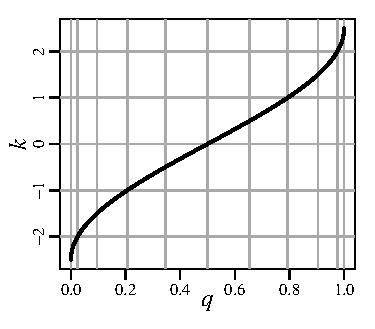
\includegraphics[width=2.5in]{figures/k-q-plot.pdf} 
   \caption{The scale function translates the quantile $q$ to the scale factor $k$ in order to give variable size steps in $q$. Limiting cluster sizes allows better accuracy near $q=0$ or $q=1$. }
   \label{fig:k-q-plot}
\end{figure}
In this figure, the horizontal lines are spaced uniformly at integer values of $k$. Vertical lines are drawn from the intersection of the scale function with these evenly spaced horizontals. The  vertical lines near $q=0$ and $q=1$ are spaced more closely,  illustrating how clusters there will be kept smaller than near the median. Proceeding from $k_0$ to $k_3$, each scale function is progressively steeper near $q=0$ and $q=1$ forcing the first and last few clusters to be progressively smaller. Scale functions $k_1$ and $k_2$ are similar, except that the value of $k$ at $q=0$ and $q=1$ is infinite. The practical impact of these infinite tails is to force the first and last cluster to have only a single sample. 
Scale function $k_0$, in contrast, is linear which results in roughly equal sized clusters.
 
Smaller clusters give smaller errors in estimating quantiles because the interpolated empirical cumulative distribution function tracks the actual empirical distribution more closely. This difference is illustrated in Figure \ref{fig:linear-interpolation}.
\begin{figure*}[htb] %  figure placement: here, top, bottom, or page
   \centering
   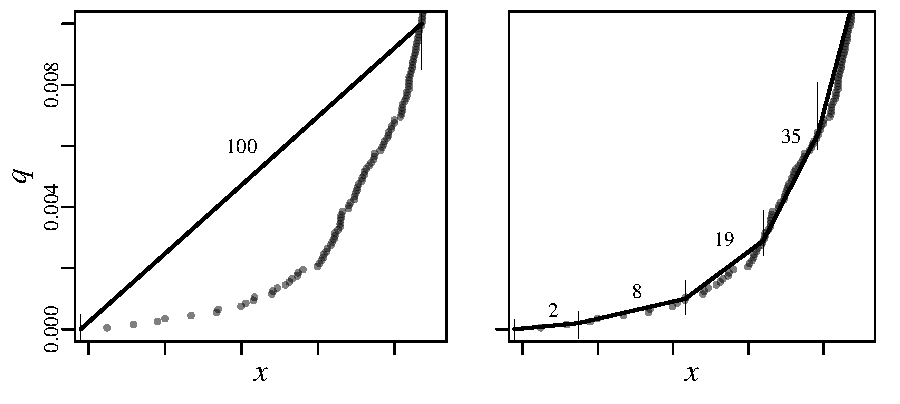
\includegraphics[height=2.in, clip]{figures/linear-interpolation.pdf} 
   \caption{The left panel shows linear interpolation of the cumulative distribution function near $q=0$ with $100$ equal sized clusters applied to $10,000$ data points sampled from an exponential distribution. The right panel shows the same interpolation with variable size clusters as given by a strongly ordered $t$-digest with $\delta=100$. The numbers above the data points represent the number of points in each cluster. Smaller clusters make interpolation more accurate.}
   \label{fig:linear-interpolation}
\end{figure*}
This figure shows roughly the first percentile of 10,000 data points sampled using $x \sim \log  \mathrm{Uniform}(0,1)$. In the left panel, the data points have been divided into 100 clusters, each with 100 data points, of which only the first bin is visible. The use of equal sized bins means that the linearly interpolated value of $q$ in the left panel of the figure has a substantial and unavoidable error. The right panel, on the other hand, shows a $t$-digest with roughly the same number of bins ($102$ instead of $100$), but with many fewer points in bins near  $q=0$. Obviously, the relationship between $x$ and $q$ can be estimated more precisely with these smaller clusters.

Of course, since every sample must be in some cluster, filling some clusters with fewer than $100$ samples requires that some other cluster or clusters must have more than $100$ samples, or we have to have more clusters. 

In the particular example shown in Figure \ref{fig:linear-interpolation}, the first bin has only 2 samples and thus zero error and the second bin has only 10 samples giving much smaller error than a cluster of $100$ samples would give. The clusters near $q=1/2$, on the other hand, have about $1.6$ times more samples than the uniform case, increasing errors by only a modest factor relative to equal sized bins. The overall effect is that quantile estimation accuracy is dramatically improved at the extremes but only modestly impaired near the median. Exactly how much accuracy at the tails is improved depends on the choice of scale function and, crucially, on how close the $t$-digest is to being strictly ordered.

\subsection{Stratified Merging}
If the clusters in a $t$-digest overlap substantially, the accuracy of the interpolated quantile estimates will be  impaired. In order to decrease that overlap, the $t$-digest library by default uses a higher value of $\delta$ while data is being added to a digest and then decreases $\delta$ when the digest is persisted. This can be done without increasing the memory requirements of the digest, but there is a cost in terms of speed since more of the memory used in the digest is devoted to clusters and less memory is used for incoming samples. That means that new data has to be merged a bit more often, and each merge takes a bit more time. In practice, the improvement in accuracy is dramatic while the cost in speed is modest, making this a good tradeoff.

The tradeoff represented in stratified merging ranges from one extreme of no stratification at all to the case where the intermediate value of $\delta$ is so large that nearly all memory is consumed by clusters and there is no room for buffered samples resulting in very large slowdown. In current implementations, a heuristic is used in which the intermediate value of $\delta$ is the geometric mean of the buffer size and the final value of $\delta$. This strategy has not been subjected to deep analysis, but  in practice it seems to be a reasonable middle ground between better accuracy and higher overhead.
\subsection{Degree of overlap of t-digest clusters}
Figure \ref{fig:cluster-spread} shows how effective the stratified merging strategy  is at producing high quality clusters. This requires about 20\% more merge operations and  each merge operation is typically less than twice as expensive. The resulting clusters are not quite strictly ordered, but overlap between clusters is limited to adjacent clusters.
\begin{figure}[htb] %  figure placement: here, top, bottom, or page
\center
   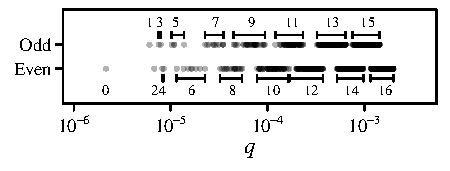
\includegraphics[width=3in]{figures/cluster-spread.pdf} 
   \caption{This typical $t$-digest is not strictly ordered, but only adjacent clusters overlap. In these first 16 clusters odd clusters overlap with adjacent even clusters, but never with adjacent odd clusters. Similarly, even clusters do not overlap with even ones. 
This corresponds to weak ordering with $\Delta=1$. Note also that the first three clusters are all singletons which drives estimation errors to zero roughly where $q < 5 \times 10^{-5}$.  }
   \label{fig:cluster-spread}
\end{figure}
The digest shown in Figure \ref{fig:cluster-spread} was produced by inserting $10^6$ samples using a working compression of $\delta = 316$ and alternating the direction of merges. The final digest was produced by doing a final merge step with $\delta = 100$, resulting in a roughly $3:1$ merge of the working clusters. With unidirectional merge steps and keeping $\delta=100$ during construction, the overlap between clusters commonly extends to the adjacent 3-4 clusters, thus degrading accuracy.
\begin{figure*}[htb] %  figure placement: here, top, bottom, or page
   \centering
   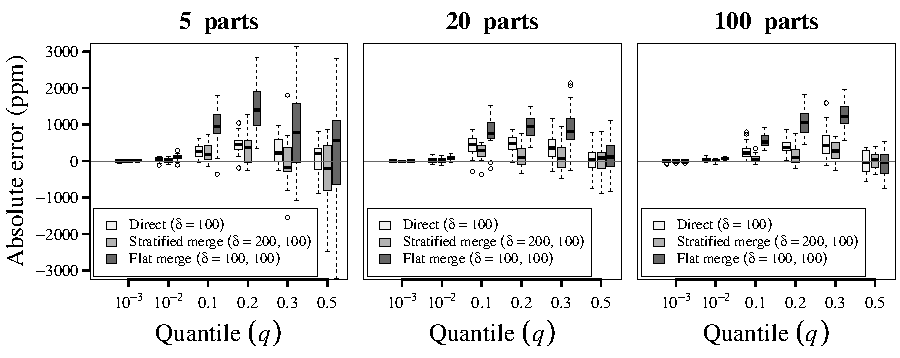
\includegraphics[width=5in]{figures/merge.pdf} 
   \caption{Accuracy of a $t$-digest formed by merging sub-digests from equal-sized partitions is as good or better than a digest accumulated on all of the data at once if the sub-digests have a larger value of $\delta$ than the final desired value. All panels were computed by 20 repetitions of aggregating 1,000,000 values.}
   \label{fig:merge}
\end{figure*}

\subsection{The clustering variant}
If we allow the buffer in the merging variant of the $t$-digest algorithm to contain just a single element so that merges can take place every time a new point is added, the algorithm takes on a new character and becomes much more like traditional $k$-means clustering than like a buffer and merge algorithm.

The basic outline of the clustering algorithm for constructing a $t$-digest is quite simple.  An initially empty ordered list of clusters $C = [ \mathcal C_1 \ldots \mathcal C_m ]$ is kept.  Each cluster is summarized by a sample mean and a count.  To add a new value $x_n$ with a weight $w_n$, the subset of centroids is found that have minimum distance to $x_n$.  This set is reduced by retaining only centroids whose $k$-size after adding $w_n$ would meet the size bound.  If more than one centroid remains, the one with maximum weight is selected.  If an acceptable centroid is found, then the new point, $(x_n,w_n)$, is added to that centroid. If no satisfactory centroid is found, then $(x_n,w_n)$ is used to form a new cluster with weight $w_n$.

Certain insertion orders can cause the number of centroids to increase without bound for this clustering algorithm. For instance, if the values of $X$ are in ascending or descending order, $C$ will contain as many centroids as samples inserted since each incoming sample will never cluster with other samples.  With scale functions other than $k_0$, this happens because each new value of $X$ is always a new maximum (or minimum) and thus will always form a new cluster and that new cluster will have maximum weight of $1$.  With $k_0$, the growth with ordered insertions is slower because as new samples are added to the largest or smallest cluster, that cluster will be allowed to grow to a weight of roughly $n/\delta$, but other clusters will never be merged and thus will stay smaller than desired. This causes the number of clusters to grow as $\Theta(\sqrt n )$. 

To avoid this pathological growth, the digest can be consolidated by making a sequential pass over all clusters to merge adjacent clusters whenever the number of clusters grows beyond a preset limit. At worst, then, the clustering variant of the $t$-digest algorithm reduces to the merging variant at the cost of maintaining a more complex data structure such as a balanced tree.

\subsection{Parallel Construction of Digests}
Digests can be constructed separately and merged to construct a digest of a large amount of data. This might be done, for example, in a time-series database where samples are processed at a very high rate. To minimize the amount of data actually stored, digests for each minute of data can be computed and stored. Each day, 1440 minute digests can be combined to form a digest for the day. Each month, the daily digests can be merged to form a monthly digest. At query time, a digest can be formed for any period of time by simply merging a few digests. For example, if we want to compute a digest for the first 100 days of a year, we would merge digests for January, February and March along with either 9 or 10 days from April (depending on whether we have a leap year).

Stratified merging is also be applied when multiple digests are merged after being constructed independently. This is done by simply using a larger value of $\delta$ when constructing the individual digests than is used for the merged result. 

\begin{figure*}[htb] %  figure placement: here, top, bottom, or page
   \centering
   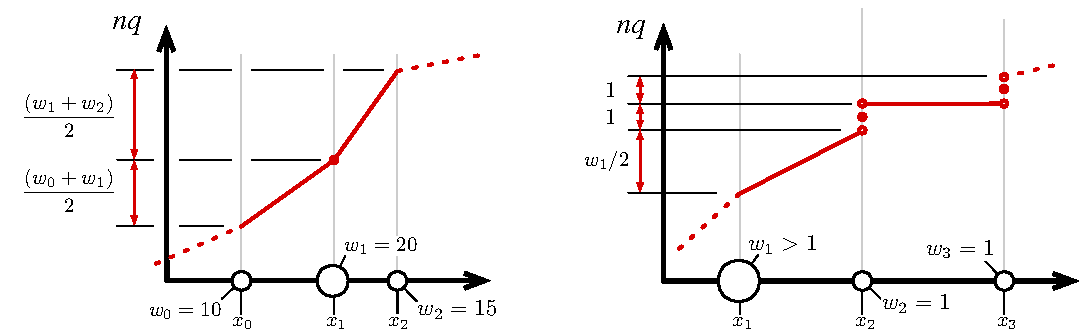
\includegraphics[width=5in]{figures/combined.pdf} 
   \caption{In the left panel, interpolation of the empirical cumulative distribution function between centroids of clusters with more than one sample is done by assuming half of the points for each centroid are to the left of the centroid and half are to the right. In the right panel, special handling for clusters with a single sample is shown. }
   \label{fig:combined}
\end{figure*}

\begin{figure}[h] %  figure placement: here, top, bottom, or page
   \centering
   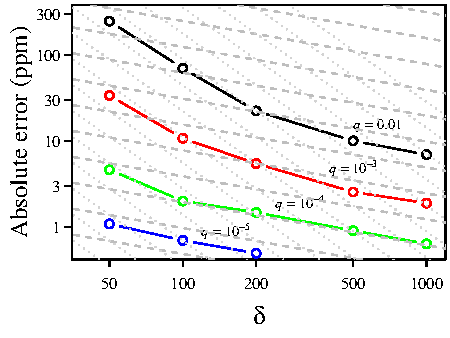
\includegraphics[width=3.in]{figures/error-vs-compression-small.pdf} 
   \caption{The scaling of quantile estimation for various values of compression factor $\delta$ and $q$ with $10^6$ samples summarized using $k_2$. 
   The general pattern is that absolute error scales like $1/\delta^2$ for small values of $\delta$ and like $1/\sqrt{\delta}$ for values larger than some cutoff. The grey dashed lines provide a reference for $1/\sqrt{\delta}$ scaling, the dotted grey lines show $1/\delta^2$ scaling.   }
   \label{fig:accuracy-scaling}
\end{figure}
\begin{figure}[h] %  figure placement: here, top, bottom, or page
   \centering
   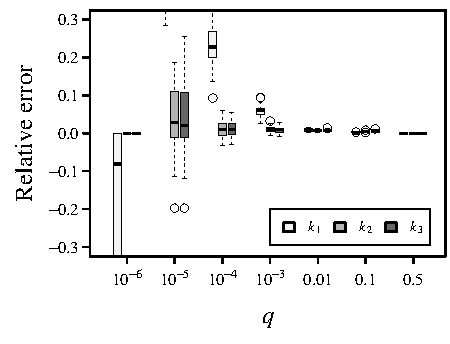
\includegraphics[width=3in]{figures/relative-error-one-panel.pdf} 
   \caption{Relative error of estimations of quantile with $\delta = 100$ for scale functions $k_1$, $k_2$ and $k_3$. Errors are computed by taking $10^6$ samples from a uniform distribution and comparing estimates from a $t$-digest against exact quantiles computed from the original samples. This was repeated 50 times to get a sense of variability.}
   \label{fig:by-scale}
\end{figure}
\begin{figure}[h] %  figure placement: here, top, bottom, or page
   \centering
   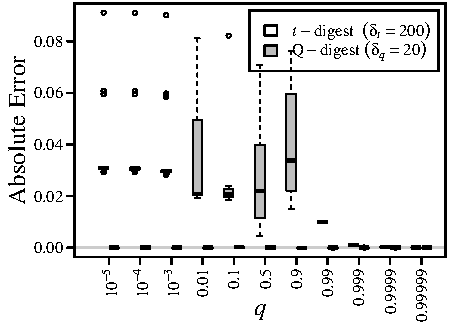
\includegraphics[width=3in]{figures/qd-sizes-small.pdf} 
   \caption{Absolute error for $t$-digest is much lower than for Q-digest with the same size digest. Here, the compression parameter for each digest was chosen to result in a serialized size of approximately 1kB. Trials with a million samples were repeated 20 times to get an idea of the variability. With this vertical scale, $t$-digest errors are not visibly different from zero.  }
   \label{fig:qd-comparison}
\end{figure}
Figure \ref{fig:merge} illustrates how this turns out. It shows accuracy achieved when summarizing 1,000,000 samples averaged over 20 experiments. The panels, taken from left to right, show the results of merging 5, 20 and 100 sub-digests. Within each panel, the three bars represent the use of a single digest which internally uses $\delta=300,100$ stratified merging, merged digests with $\delta=300$ in the sub-digests and $\delta=100$ in the final result and a non-stratified merge with $\delta=100$ at both levels. At all levels of parallelism, the non-stratified merge result is the worst for accuracy. Stratified parallel merging was comparable to the non-parallel merge though a bit more variable with 5-way parallelism and progressively more accuracy with more parallelism.


In terms of speed, merging $t$-digests is fairly fast relative to practical requirements. In one experiment, 1000 digests were used to summarize 1,000,000 samples each and these digests were then merged into a single digest. It took about 150ms to fill each digest and about 150 ms to merge all thousand digests. Each digest is about 1kB in serialized form in this example so a total of about 1 MB of digests must be processed by the merge. Overall, this means that, with sufficient hardware (roughly 1000 cores), a $t$-digest can be produced from a billion data points in less than half a second. The cost of merging $t$-digests is, nevertheless, higher than the cost of merging some other kinds of sketches such as the moment sketches discussed later.

\subsection{Interpolation}
Accurate interpolation of the empirical distribution function is critical to the accuracy of quantile estimation with the $t$-digest. In general, interpolation proceeds by assuming that half of the mass of any cluster is to the left of the cluster centroid and half is to the right. We also assume that the data between adjacent centroids is uniformly distributed. These assumptions allow us to linearly interpolate the mass of adjacent clusters as is shown in the left panel of Figure \ref{fig:combined}. 

Special cases that arise when clusters have only a single sample as is common with the first or last few centroids are shown in the right panel of Figure \ref{fig:combined}. In particular, retaining the minimum and maximum values is equivalent to forcing the first and last clusters to have a single sample.


\section{Size/Accuracy Trade-off}
Not surprisingly, there is a trade-off between the size of the $t$-digest as controlled by the compression parameter $\delta$ versus the accuracy of quantile estimation.  Figure \ref{fig:accuracy-scaling} shows the trade-off for different quantiles with $10^6$ samples from a uniform distribution. The same trade-off applies symmetrically for values of $\delta$ near 1 as well.

As can be seen, the commonly used values of $\delta=100$ or  $\delta=200$ relative accuracy of 10\% or better. With $\delta=200$, relative accuracy is commonly 1\%.

Figure \ref{fig:by-scale} examines the accuracy of quantile estimation with a $t$-digest for different scale functions.  As intended, absolute error in quantile estimation is small and decreases near $q=0$ and $q=1$ (left panel) for scale functions $k_1$, $k_2$ and $k_3$. Though it is hard to see in this figure because of the vertical scale, in the mid-range where $q \in [0.1, 0.9]$, $k_1$ provides somewhat better absolute error than $k_2$ and $k_3$. 


All scale functions show a pattern of decreasing absolute error for more and more extreme values of $q$, but $k_2$ and $k_3$ achieve single digit part per million errors for $q\le 0.001$ or $q\ge0.999$, which is surprisingly good since only about 50 to 60 centroids are retained in total for $\delta=100$. 

For most applications, we have seen that $\delta=100$ provides sufficient accuracy and scale function $k_2$ or $k_3$ provide a good combination of relative and absolute error. Values as low as $\delta=20$ may be useful, especially if $k_0$ is used to get uniform absolute error. At this level, the persisted size of the digest is about 200 bytes and errors are uniform at about 1\%.

\subsection{Comparison with Q-digest}
In terms of error size, the 4.0 preview implementation of $t$-digest dominates the implementation of the Q-digest from the popular stream-lib package \cite{qdigest,github:stream} when digests of the same size are compared.  This is shown in Figure \ref{fig:qd-comparison}.  In the left panel, the relationship between the compression parameter $q$ and size is shown for both digests for 20 trials where 100,000 uniformly distributed samples are inserted into each kind of digest.  To force the digests to be equal in size, compression parameter values of $\delta_q=20$ for Q-digest  and $\delta_t = 200$ for $t$-digest were chosen. This gives an average digest size of about $874$ bytes for Q-digest and 990 bytes for $t$-digest, as shown in the left panel. The panel on the right compares errors under these conditions and shows that the $t$-digest errors are more than two orders of magnitude smaller for all values of $q$. For values near $q=0$ the $t$-digest produces absolute errors 3-5 orders of magnitude smaller than the Q-digest does. Relative errors are 5 or more orders of magnitude small with the $t$-digest. When compared on distributions with high amounts of skew, the results are even more striking in favor of the $t$-digest because of the limited resolution of the integer data used by the $t$-digest.

Note that the parameters chosen for this comparison depend on the number of samples because with constant $\delta$, the size of the Q-digest increases roughly logarithmically with the number of samples while the size of the $t$-digest is strictly bounded and is nearly constant once the number of samples exceeds $2 \delta$. 

\section{Conclusion}
The $t$-digest is a novel on-line sketching algorithm that dominates previous previous sketching algorithms in terms of accuracy and size particularly when considering relative accuracy for extreme quantiles.  The $t$-digest can provide accurate on-line estimates of a variety of of rank-based statistics including quantiles and trimmed mean. The core ideas of the algorithm are simple and the algorithm empirically demonstrates high accuracy even with pathological distributions.  The $t$-digest can also be used in parallel applications or in OLAP-style indexes.  

Though not previously described in published literature, the $t$-digest has already been adopted widely by companies such as Facebook, Microsoft and Netflix for internal monitoring and has been included in open source libraries such as Apache Mahout and stream-lib and has been incorporated into prominent open-source projects such as Apache Lucene and Elasticsearch.

\section{Reference Implementation}
The $t$-digest algorithm is available in the form of an open source, well-tested implementation maintained the author \cite{t-digest-project}.  That distribution contains extensive unit and quality tests that exercise the system on a wide variety of distributions, particularly including mixed discrete/continuous distributions, distributions with large offsets and very highly skewed distributions.

Other implementations are available in C++, Go, Python and Javascript.

\section{Acknowledgments}
This paper was prepared with the gracious assistance of Ellen Friedman who reviewed and provided helpful feedback.
%\subsection{}
\bibliographystyle{abbrv}
\bibliography{refs}{}

\end{document}  
